% =====================================================================
%  SchemaLens V3: Stage 7/8 unificado (trabalho físico estrutural + Pareto)
%  avaliado em IoT-Benchmark, TPCx-IoT, TSBS cpu-only e RUBiS.
%  Compilar no Overleaf com pdfLaTeX. Tabelas/figuras geradas por build_tables.py
%  a partir de outputs_v3/ (nenhum número de tabela é digitado à mão).
% =====================================================================
\documentclass[10pt,a4paper,twoside]{article}
\usepackage[T1]{fontenc}
\usepackage[utf8]{inputenc}
\usepackage{lmodern}
\IfFileExists{brazil.ldf}{\usepackage[brazil]{babel}}{}
\usepackage[a4paper,margin=2.0cm]{geometry}
\usepackage{amsmath,amssymb,amsthm}
\usepackage{graphicx,booktabs,tabularx,longtable,array,float}
\usepackage[font=small,labelfont=bf]{caption}
\usepackage[table]{xcolor}
\usepackage{microtype}
\IfFileExists{enumitem.sty}{\usepackage{enumitem}\setlist{itemsep=1pt,topsep=2pt}}{}
\usepackage[colorlinks=true,linkcolor=blue!50!black,urlcolor=blue!50!black,citecolor=green!40!black]{hyperref}
\emergencystretch=3em
\newcolumntype{Y}{>{\raggedright\arraybackslash}X}
\makeatletter\newcommand{\tabin}[1]{\@@input #1 }\makeatother
\definecolor{boxbg}{RGB}{243,246,250}
\newcommand{\caixa}[1]{\par\smallskip\noindent\colorbox{boxbg}{\parbox{\dimexpr\linewidth-2\fboxsep}{#1}}\par\smallskip}
\theoremstyle{definition}\newtheorem{definicao}{Definição}
\newcommand{\tsbsRankOneNat}{0,548}
\newcommand{\tsbsRankOneNatLo}{0,529}
\newcommand{\tsbsRankOneNatHi}{0,568}
\newcommand{\tsbsRankOneAli}{0,379}
\newcommand{\tsbsFloorNat}{12,3}
\newcommand{\tsbsFloorAli}{4,9}
\newcommand{\tsbsTiedNat}{23}
\newcommand{\tsbsRaw}{49.920}
\newcommand{\iotFloor}{2,15}
\newcommand{\tpcxFloor}{6,13}
\newcommand{\tpcxTied}{6}
\newcommand{\rubisOracle}{v311: 3577311/3577311; v41: 3577311/3577311}
\newcommand{\rubisTauVer}{bidding 0,56, browsing 0,78, update100x 0,00, update10x 0,89}


\title{\textbf{SchemaLens V3: um Stage 7 único para quatro benchmarks}\\[3pt]
\large Estimativa estrutural de trabalho físico, Pareto universal e preservação de alternativas competitivas no Apache Cassandra}
\author{Projeto SchemaLens / Cassandra}
\date{V3 --- novembro de 2026}

\begin{document}
\maketitle

\begin{abstract}
\noindent Na versão anterior (V2) do SchemaLens, a fase de medição já seguia um protocolo comum. A etapa que estima custos e
escolhe o HBench (Stage 7/8), porém, era diferente em cada benchmark: fatores de custo por família no IoT-Benchmark,
cenários ilustrativos fora da escala executada no TPCx-IoT e no TSBS, e um modelo de latência calibrado por mínimos
quadrados não negativos (NNLS) no RUBiS. Este artigo apresenta a \textbf{V3}, que substitui essas quatro variantes por um
único módulo, com o mesmo modelo de dados, a mesma estimativa de \emph{trabalho físico estrutural}, a mesma semântica de
viabilidade, a mesma dominância de Pareto em seis eixos e a mesma regra de diversidade e desempate. A estimativa não usa
latência, não tem coeficientes por família e não tem escore escalar. O cenário de cada Stage 7 passa a ser o da campanha
realmente executada. O HBench é congelado por SHA-256 e pré-registrado antes de qualquer execução no Cassandra, e um
firewall impede que a seleção leia resultados medidos.

\noindent Seguindo a regra de reutilização definida para esta versão, remedimos apenas os benchmarks cujo HBench mudou:
\begin{itemize}
\item TSBS: verificação completa dos 24 deployments V3, mais o esquema original e uma réplica A/A;
\item RUBiS: Cassandra 4.1.12 e 3.11.11.
\end{itemize}
No IoT-Benchmark e no TPCx-IoT o HBench V3 já tinha sido medido na V2 com as mesmas rotas, e por isso as medições foram reanalisadas.

\noindent Resultados:
\begin{itemize}
\item O espaço foi reduzido em 67\% a 98\%.
\item Em todos os benchmarks o HBench V3 contém o melhor deployment medido ou um empatado com ele pelo piso de ruído A/A, com regret de 0 a 1,7\%.
\item O rank~1 do TSBS gasta \tsbsRankOneNat$\times$ o tempo do esquema original do TSBS (\tsbsRankOneAli$\times$ na coorte alinhada).
\item No RUBiS 4.1.12, o melhor membro do HBench é 23\% a 29\% mais rápido que NoSE e QPG nas cargas de leitura e mistas, com os mesmos vereditos em 3.11.11 e 100\% de concordância com o oráculo.
\end{itemize}
Há também perdas, discutidas no texto:
\begin{itemize}
\item a ordenação estrutural não prediz latência ($\tau$ entre $-0{,}34$ e $1{,}0$, comparável ao NNLS legado avaliado retrospectivamente);
\item a retenção da fronteira medida de três objetivos cai no TPCx-IoT;
\item a regra de diversidade admitiu um deployment lento no RUBiS.
\end{itemize}
\end{abstract}

\tableofcontents
\bigskip

% =====================================================================
\section{Motivação: o que a V2 tinha de heterogêneo}
\label{sec:motivacao}

O SchemaLens tem duas fases separadas por um firewall:
\begin{itemize}
\item a fase de \emph{projeto} ativa famílias de estruturas por regras sobre o workload, instancia candidatos (CandidateSpec), sintetiza rotas de leitura (QueryPlan) e de escrita (WritePlan), estima custos (Stage 7) e escolhe deployments completos (Stage 8), formando o HBench;
\item a fase de \emph{medição} executa no Cassandra o HBench, os baselines e controles, sob um protocolo comum.
\end{itemize}
A auditoria da V2 (\texttt{docs/V3\_STAGE7\_AUDIT.md}) mostrou que a fase de medição era comum, mas o Stage 7/8 não era:

\begin{itemize}
\item \textbf{IoT-Benchmark:} pré-seleção ponderada (0,8 leitura / 0,1 armazenamento / 0,1 escrita) sobre proxies do
catálogo Rev3; em outro ramo do pipeline, fatores de leitura por família (TS0 = 1,0; TS2 = 0,62; TS4 = 0,12, ...).
\item \textbf{TPCx-IoT:} cenário ilustrativo de 10 estações $\times$ 200 sensores, horizonte de 1 dia e RF~2, enquanto a
campanha executada tinha 2 estações $\times$ 3 sensores e RF~1.
\item \textbf{TSBS:} cenário de 100 hosts, 60~s e 3 dias, enquanto a campanha executada tinha 40 hosts, 600~s e 36~h;
escore ponderado; dois perfis (conservador e alinhado condicional) com top-5 cada.
\item \textbf{RUBiS:} modelo de latência calibrado por NNLS em medições anteriores ($a_{read}=0{,}462$~ms,
$b_{write}=0{,}389$~ms, $c_{row}=0{,}0075$~ms) dentro de um ILP, com estatísticas em escala completa (2~M itens, 20~M
lances) enquanto a campanha usa uma coorte.
\end{itemize}

\caixa{\textbf{Pergunta da V3.} Um Stage 7 universal, baseado apenas em trabalho físico observável antes do benchmark,
consegue reduzir o espaço de projeto e \emph{preservar} as alternativas empiricamente competitivas, sem coeficientes de
latência específicos de dataset? A pergunta \emph{não} é se o modelo prevê exatamente quem será mais rápido: Kendall
$\tau$ é apenas diagnóstico retrospectivo e não é maximizado.}

% =====================================================================
\section{Método V3}
\label{sec:metodo}

\subsection{Arquitetura comum}
{\sloppy O módulo \texttt{unified\_stage7\_v3/} é o mesmo para os quatro benchmarks. Os \emph{adaptadores}
(\texttt{adapters/\{iot,tpcx\_iot,tsbs,rubis\}.py}) só convertem os artefatos congelados de cada benchmark para o modelo
canônico: nenhum peso, nenhum fator de família e nenhuma constante de custo vive neles.\par}

\begin{center}\small
\resizebox{\linewidth}{!}{\begin{tabular}{l}
\toprule
IoT, TPCx-IoT, TSBS, RUBiS $\;\to\;$ adaptadores $\;\to\;$ CandidateSpec, QueryPlan(AccessStep), WritePlan, Workload\\
$\to$ \textbf{UnifiedStage7Estimator}: ReadWork, WriteWork, Footprint $\;\to\;$ agregação por deployment: \textbf{PhysicalWorkVector}\\
$\to$ cobertura e viabilidade $\;\to\;$ \textbf{Pareto} (6 eixos) $\;\to\;$ diversidade estrutural $\;\to\;$ \textbf{HBench V3}\\
$\to$ congelamento por SHA-256 e pré-registro $\;\to\;$ Cassandra 4.1.12 (protocolo v1) $\;\to\;$ análise\\
\bottomrule
\end{tabular}}
\end{center}

\subsection{Estimativa estrutural de trabalho físico}
\begin{definicao}[ReadWork]
Para cada execução de um QueryPlan, com passos de acesso $s$:
\emph{read\_cql\_requests} $=\sum_s r_s$, \emph{partitions\_touched} $=\sum_s p_s$,
\emph{logical\_rows} $=\sum_s \ell_s$ e \emph{logical\_bytes} $=\sum_s \ell_s\, w(\text{colunas projetadas de }s)$;
o \emph{fan-out} é o número de partições dividido pelo número de operandos lógicos da consulta.
\end{definicao}
\begin{definicao}[WriteWork e Footprint]
Por execução de uma escrita e por tabela mantida: \emph{cql\_mutations}, \emph{rows\_touched},
\emph{maintenance\_read\_requests}, \emph{maintenance\_rows\_read} e \emph{logical\_bytes\_written}. As leituras de suporte
compartilhadas pelas tabelas de uma mesma escrita contam uma vez por (escrita, entidade). Por candidato:
\emph{logical\_storage\_bytes} $=$ linhas $\times$ largura, número de partições, maior partição em linhas e em bytes, e
razão de duplicação.
\end{definicao}

A política de bytes lógicos \textbf{LBP-1} é comum e versionada:
\begin{itemize}
\item larguras fixas por tipo CQL (\texttt{bigint} 8, \texttt{double} 8, \texttt{int} 4, \texttt{uuid} 16, \texttt{timestamp} 8, \ldots);
\item tipos variáveis usam a largura média declarada ou estimada nos dados pré-benchmark da própria campanha;
\item sem largura conhecida, a quantidade fica explicitamente \texttt{UNKNOWN} (nunca zero) e bloqueia afirmações de dominância.
\end{itemize}
Esses valores não são bytes de disco, de rede ou de SSTable. Por isso usamos os nomes \emph{logical\_bytes\_proxy} e
\emph{logical\_storage\_bytes\_proxy}.

\subsection{Rotas, viabilidade e vetor por deployment}
Dentro de um deployment, cada operação usa a \textbf{regra de rota universal}: entre os planos válidos cujas tabelas
estão todas no deployment, o mínimo lexicográfico de (requisições, linhas, bytes, identificador do plano). As guardas de
execução são avaliadas por instância. Por exemplo, no TSBS uma tabela de \emph{rollup} só é válida quando a janela da
instância está alinhada.

Um deployment é viável quando:
\begin{enumerate}
\item toda leitura tem rota;
\item toda tabela afetada por uma escrita é mantível e tem tabela de suporte;
\item existe uma fonte canônica;
\item nenhuma tabela derivada está morta, isto é, sem servir a nenhuma rota escolhida nem a leitura de suporte (D-V3-007);
\item as regras estruturais herdadas são respeitadas: no RUBiS, \emph{supersedes} e a existência de uma cópia completa de cada entidade inserida.
\end{enumerate}

O \textbf{PhysicalWorkVector} agrega as leituras pela frequência normalizada, as escritas pela frequência e pela soma
sobre as tabelas mantidas, e o armazenamento pela soma sobre os candidatos. Os riscos de partição entram como máximos.
O Stage 7 V3 \emph{não} calcula escore escalar nem latência estimada.

\subsection{Stage 8 V3: Pareto, diversidade e desempate}
A dominância de Pareto (minimização) usa seis eixos:
\begin{itemize}
\item \emph{read\_cql\_requests}, \emph{read\_logical\_rows} e \emph{read\_logical\_bytes};
\item \emph{write\_cql\_mutations} e \emph{maintenance\_read\_requests};
\item \emph{logical\_storage\_bytes}.
\end{itemize}
Os eixos de risco (maior partição em bytes e em linhas, número de partições) ficam fora da dominância. A análise
preliminar, feita só com vetores, mostrou que incluí-los faria a fronteira cobrir 100\% do espaço do IoT e 56\% do TPCx
(D-V3-006).

Se a fronteira cabe em $k=5$, ela é mantida inteira. Caso contrário, aplica-se uma seleção gulosa por \emph{tags}
estruturais (fonte canônica, tabela física, combinação de famílias, bucket, projeção ou não, dado bruto ou agregado),
e a ordem final é dada pelo
\[
\textit{balanced\_structural\_tiebreak}(d) \;=\; \frac{1}{|A|}\sum_{a\in A}\frac{v_a(d)}{\min_{d'}\{v_a(d')>0\}},
\]
com pesos iguais e mínimo tomado no espaço pré-benchmark. Esse valor serve apenas para ordenar e desempatar e não é uma
previsão de latência. O algoritmo de busca pode variar (enumeração exata nos quatro casos, até $2^{15}$ subconjuntos no
RUBiS), mas a semântica não varia.

\subsection{Firewall e congelamento}
O Stage 7/8 roda sob um interceptador de leitura de arquivos. Ele aborta ao encontrar caminhos com padrões de resultado
medido (\texttt{raw\_latencies}, \texttt{stage9}, \texttt{p95}, \texttt{E20\_benchmark}, \texttt{COST\_MODEL.json}, \ldots) e
grava no manifesto a lista dos arquivos abertos, junto com \texttt{selection\_uses\_measured\_results=false}.

O congelamento faz três coisas:
\begin{itemize}
\item calcula o SHA-256 do código V3, das entradas, das saídas 00--12, do cenário, do protocolo e do \emph{harness};
\item reexecuta o Stage 7/8 em um processo novo e exige saídas idênticas byte a byte;
\item grava o pré-registro.
\end{itemize}
Todo ponto de entrada do Stage 9 chama \texttt{verify()} e aborta se qualquer hash mudar. Quinze testes obrigatórios,
somando 41 casos, cobrem: firewall, irrelevância de \emph{query ids} e de rótulos de família, plano igual gerando vetor
igual, quantidades finitas e não negativas, \texttt{UNKNOWN} explícito, ausência de fator por família, cenário igual ao
executado, invalidação do congelamento, cobertura de corretude e inalcançabilidade do NNLS legado.

% =====================================================================
\section{Cenários, frequências e volumes}
\label{sec:cenarios}

O cenário do Stage 7 V3 é o da campanha executada (D-V3-003, arquivo \texttt{V3\_PREBENCHMARK\_SCENARIO.json}):

\begin{table}[H]\centering\small
\caption{Cenário V3 de cada benchmark (igual ao medido) e cenário antigo descartado.}
\begin{tabularx}{\linewidth}{lYY}
\toprule
Benchmark & Cenário V3 (= campanha executada) & Cenário antigo do Stage 7 \\
\midrule
IoT-Benchmark & campanha B Rev3: 9 dispositivos, 54\,000 células métricas, 12 consultas (janela de 7 dias), mesmo CSV medido & --- (fatores por família) \\
TPCx-IoT & 2 estações $\times$ 3 sensores, 130 + 500 passos de 1~s, 3\,780 eventos e 120 leituras de 2 janelas por execução, \emph{padding} de 900~B, RF~1 & 10 $\times$ 200, 1 dia, RF 2 \\
TSBS cpu-only & gerador Go oficial (commit 8323e59c): 40 hosts, 600~s, 36~h, 8\,640 observações / 86\,400 células; 96 instâncias congeladas (16 \emph{templates} $\times$ 3 $\times$ coortes natural e alinhada) & 100 hosts, 60~s, 3 dias \\
RUBiS & estado da coorte congelada: 7\,392 itens, 5\,690 lances, 6\,529 comentários, 5\,300 compras, 21\,855 usuários (com fechamento), 500 categorias, 50 regiões; estatísticas E04 recalculadas com \emph{fan-outs} no domínio de parâmetros das histórias & escala completa: 2~M itens, 20~M lances; NNLS \\
\bottomrule
\end{tabularx}
\end{table}

As frequências só são usadas quando têm fonte legítima anterior ao benchmark:
\begin{itemize}
\item IoT: \texttt{EXPERIMENTAL\_POLICY\_UNIFORM} sobre Q1--Q12;
\item TPCx: os parâmetros congelados do workload (120 leituras e 3\,780 ingestões por execução);
\item TSBS: \texttt{UNSPECIFIED} com \texttt{UNIFORM\_QUERY\_CLASS};
\item RUBiS: as frequências por instrução da E05, agregadas pela média das quatro cargas (D-V3-009).
\end{itemize}

% =====================================================================
\section{Resultado pré-benchmark: o novo HBench}
\label{sec:pre}

\begin{table}[H]\centering\small
\caption{Espaço de projeto e HBench V2 $\times$ V3 (identidade = conjunto de tabelas). A última coluna aplica a regra
D-V3-001: só se mede de novo quando o conjunto a medir contém (tabelas, rotas) não medidos na V2.}
\label{tab:espaco}
\begin{tabular}{lrrrrrrrrl}
\toprule
Benchmark & cand. & enumer. & viáveis & Pareto & $|H_{V2}|$ & $|H_{V3}|$ & $\cap$ & Jaccard & medição \\
\midrule
\tabin{tables/space.tex}
\bottomrule
\end{tabular}
\end{table}

Os quatro HBench V3 aparecem com seus vetores físicos (tabelas~\ref{tab:hiot}--\ref{tab:hrubis}). Pontos principais:
\begin{itemize}
\item \textbf{IoT:} a fronteira tem um ponto só, TS2-U (tabela larga sem bucket), que domina TS0 e TS2-D. A tabela
\emph{latest} TS4 é morta, pois a rota lexicográfica nunca a escolhe, e por isso não entra.
\item \textbf{TPCx:} a fronteira é \{TS0, TS0+TS3-3600\}. A projeção TS3 por sensor troca 4 requisições por 2 ao custo
de dobrar as escritas e o armazenamento.
\item \textbf{TSBS:} 7 pontos na fronteira; a diversidade escolhe 5, todos com a dimensão por hora TS6.
\item \textbf{RUBiS:} 20 pontos na fronteira de 256 deployments viáveis. A diversidade mantém H01, H02 e H04 da V9/V2,
com rotas idênticas, e acrescenta dois deployments inéditos: V3H02 (= H01 + \texttt{C015}) e V3H05
(\texttt{C005}, \texttt{C008}, \texttt{C013}, \texttt{C015}).
\end{itemize}

\newcommand{\hbhead}{\# & deployment & req. & linhas & bytes & mutações & leit. manut. & armaz. (KiB) & tiebreak\\\midrule}
\begin{table}[H]\centering\scriptsize
\caption{HBench V3 do IoT-Benchmark (vetor por execução do mix; mutações = carga estática).}\label{tab:hiot}
\begin{tabular}{rlrrrrrrr}\toprule\hbhead\tabin{tables/hbench_iot.tex}\bottomrule\end{tabular}
\end{table}
\begin{table}[H]\centering\scriptsize
\caption{HBench V3 do TPCx-IoT (por leitura lógica; mutações por execução).}\label{tab:htpcx}
\begin{tabular}{rlrrrrrrr}\toprule\hbhead\tabin{tables/hbench_tpcx_iot.tex}\bottomrule\end{tabular}
\end{table}
\begin{table}[H]\centering\scriptsize
\caption{HBench V3 do TSBS (média por instância das 96; mutações da carga).}\label{tab:htsbs}
\begin{tabular}{rlrrrrrrr}\toprule\hbhead\tabin{tables/hbench_tsbs.tex}\bottomrule\end{tabular}
\end{table}
\begin{table}[H]\centering\scriptsize
\caption{HBench V3 do RUBiS (média das 4 cargas E05 por requisição; entre parênteses, as tabelas além das 9 obrigatórias).}\label{tab:hrubis}
\resizebox{\linewidth}{!}{\begin{tabular}{rlrrrrrrr}\toprule\hbhead\tabin{tables/hbench_rubis.tex}\bottomrule\end{tabular}}
\end{table}

\paragraph{Por que remedir TSBS e RUBiS.}
\begin{itemize}
\item \textbf{TSBS:} as tabelas do HBench V3 já tinham sido medidas na V2, mas em duas implantações (as que contêm
TS5hh) a regra de rota universal manda 5 instâncias alinhadas para TS0. Quando a janela cruza a fronteira de um dia,
TS5hh precisa de 2 requisições por host e TS0 de 1. A regra foi declarada antes dessa observação e não foi ajustada
(D-V3-008).
\item \textbf{RUBiS:} V3H02 e V3H05 nunca tinham sido medidos.
\end{itemize}

% =====================================================================
\section{Protocolo de medição}
\label{sec:protocolo}

O protocolo comum v1 da V2 foi mantido sem alteração:
\begin{itemize}
\item imagem \texttt{cassandra@sha256:25f6a4d5\ldots} (4.1.12) em contêiner dedicado (cpuset 0--3, 6~GB, heap 2~GB), RF~1;
\item 5 repetições com reinício a frio, \emph{gate} de flush (SSTable $\geq 1$, memtable vazia) e guarda de isolamento/compactação;
\item ordem contrabalançada e oráculo independente em cada resposta cronometrada;
\item média como métrica de decisão; p50, p95 e p99 por posto exato;
\item \emph{bootstrap} pareado estratificado ($B=2000$) e piso de ruído pela réplica A/A;
\item armazenamento medido após o flush.
\end{itemize}

Por benchmark:
\begin{itemize}
\item \textbf{TSBS:} verificação completa (os 24 deployments V3, o esquema original \texttt{series\_bigint} e a réplica
A/A do rank~1, somando 26 variantes); 2 aquecimentos e 12 rodadas por repetição (desvio declarado na V2, mantido);
\tsbsRaw{} medições cronometradas.
\item \textbf{RUBiS:} dois nós \emph{novos} (4.1.12 principal e 3.11.11 secundário), criados só para a V3; HBench V3,
NoSE, QPG, V8-norm e a réplica A/A V3H01\_AA; histórias semeadas idênticas às da V9 (1\,000 aquecimentos e
10\,000 requisições por carga, deployment, repetição e versão).
\item \textbf{IoT e TPCx:} reanálise das latências brutas da campanha V2, que mediu todo o espaço V3 com rotas idênticas.
\end{itemize}
Antes do congelamento, \emph{smokes} do TSBS e do RUBiS validaram os \emph{harnesses}.

% =====================================================================
\section{Resultados}
\label{sec:resultados}

\subsection{Quadro geral V2 $\times$ V3}
\begin{table}[H]\centering\small
\caption{Métricas de método. Top-1 (ruído) = o rank~1 do seletor empata com o melhor medido pelo piso A/A. Regret =
melhor do HBench / melhor do espaço $-$ 1. Retenção = fração da fronteira medida (leitura $\times$ armazenamento
$\times$ escrita) que está no HBench. $\tau$ = Kendall entre o escore do seletor e a média medida (diagnóstico).
TSBS: V2 e V3 são campanhas diferentes (espaço medido de 10 e de 24).}
\label{tab:metricas}
\resizebox{\linewidth}{!}{\begin{tabular}{lrrcccrrr}
\toprule
seletor & HBench/espaço & DSR & Top-1 estrito & Top-1 (ruído) & Top-3 & regret & retenção Pareto & $\tau$ \\
\midrule
\tabin{tables/metrics.tex}
\bottomrule
\end{tabular}}
\end{table}

\subsection{IoT-Benchmark e TPCx-IoT (reanálise)}
\begin{table}[H]\centering\scriptsize
\caption{IoT-Benchmark: espaço V3 completo, medido na V2. Piso A/A = \iotFloor\%.}
\begin{tabular}{lccrrrrcr}\toprule
deployment & $H_{V3}$ & $H_{V2}$ & média (ms) & IC 95\% & armaz. (KiB) & carga (s) & empata & tiebreak\\\midrule
\tabin{tables/space_iot.tex}\bottomrule\end{tabular}
\end{table}
\begin{table}[H]\centering\scriptsize
\caption{TPCx-IoT: os 9 deployments V3, medidos na V2 durante ingestão concorrente. Piso A/A = \tpcxFloor\%; \tpcxTied{} empatam com o melhor.}
\begin{tabular}{lccrrrrcr}\toprule
deployment & $H_{V3}$ & $H_{V2}$ & média (ms) & IC 95\% & armaz. (KiB) & ingestão (s) & empata & tiebreak\\\midrule
\tabin{tables/space_tpcx_iot.tex}\bottomrule\end{tabular}
\end{table}

\textbf{IoT-Benchmark.} O único deployment retido é o melhor medido, com redução de 3 para 1, sem perda de preservação.

\textbf{TPCx-IoT.}
\begin{itemize}
\item Os seis deployments com projeção TS3 empatam a $\approx$2,9~ms; TS0 e TS1 ficam a $\approx$4,6--5,1~ms.
\item O HBench V3 tem um representante do grupo rápido (TS0+TS3-3600, a 0,17\% do melhor), mas o desempate estrutural
coloca TS0 em primeiro lugar, porque tem menos escritas e menos armazenamento. Por isso o Top-1 falha e a retenção da
fronteira medida cai para 33\%.
\end{itemize}

\subsection{TSBS cpu-only (nova campanha, verificação completa)}
\begin{figure}[H]\centering
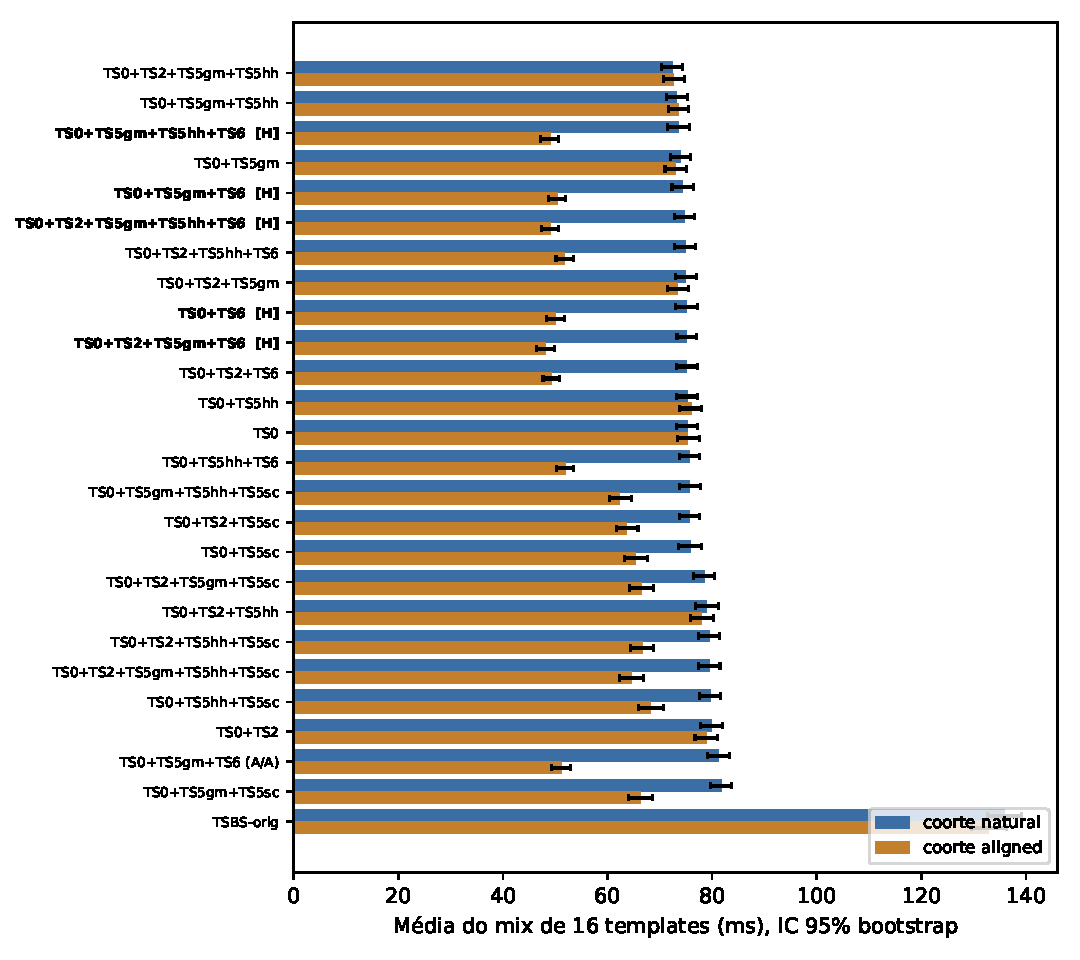
\includegraphics[width=0.82\linewidth]{figs/tsbs_v3.pdf}
\caption{TSBS: média do mix (IC 95\%) das 26 variantes nas duas coortes; [H] marca o HBench V3.}
\label{fig:tsbs}
\end{figure}
\begin{table}[H]\centering\scriptsize
\caption{TSBS: as 26 variantes ordenadas pela coorte natural.}
\resizebox{\linewidth}{!}{\begin{tabular}{lcrrrrrrr}\toprule
deployment & $H_{V3}$ & natural (ms) & IC 95\% & p95 nat. & alinhada (ms) & IC 95\% & armaz. (KiB) & carga (s)\\\midrule
\tabin{tables/tsbs_variants.tex}\bottomrule\end{tabular}}
\end{table}

\textbf{Coorte natural} (janelas TSBS arbitrárias):
\begin{itemize}
\item O piso A/A é alto (\tsbsFloorNat\%): \tsbsTiedNat{} dos 24 deployments empatam com o melhor.
\item O HBench contém deployments empatados, com regret de 1,7\%.
\end{itemize}

\textbf{Coorte alinhada} (onde as tabelas de \emph{rollup} servem):
\begin{itemize}
\item O piso A/A é \tsbsFloorAli\%.
\item O melhor medido (TS0+TS2+TS5gm+TS6, a 48,2~ms) está no HBench, com regret 0.
\item Os deployments com TS6 ficam em 48--52~ms, contra 73--79~ms sem TS6.
\end{itemize}

\textbf{Contra o esquema original do TSBS:} o rank~1 V3 gasta \tsbsRankOneNat{} [\tsbsRankOneNatLo; \tsbsRankOneNatHi]
$\times$ o tempo do original na coorte natural e \tsbsRankOneAli$\times$ na alinhada.

\subsection{RUBiS (nova campanha, 4.1.12 e 3.11.11)}
\begin{figure}[H]\centering
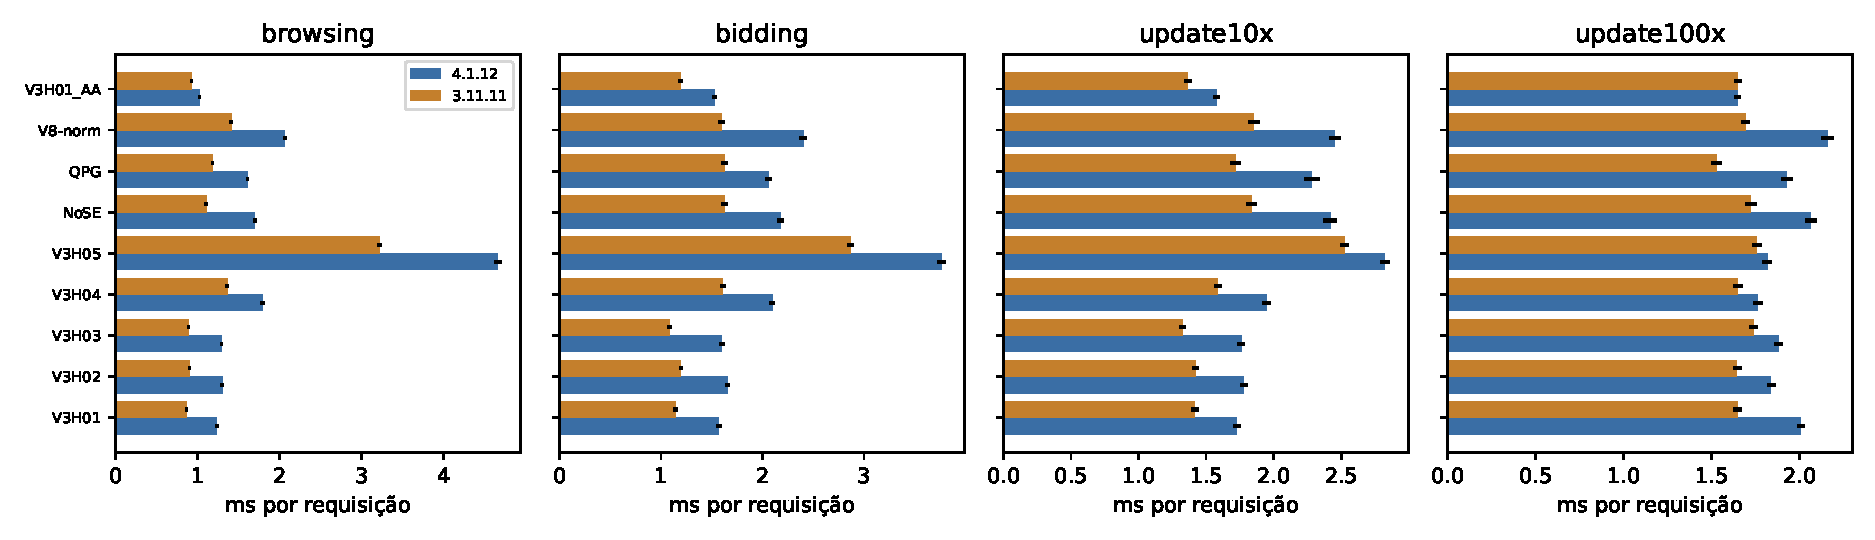
\includegraphics[width=\linewidth]{figs/rubis_v3.pdf}
\caption{RUBiS: latência média por requisição (IC 95\%) nas quatro cargas e nas duas versões.}
\label{fig:rubis}
\end{figure}

\newcommand{\rubhead}{deployment & \multicolumn{2}{c}{browsing} & \multicolumn{2}{c}{bidding} & \multicolumn{2}{c}{update10x} & \multicolumn{2}{c}{update100x}\\ & média & p95 & média & p95 & média & p95 & média & p95\\\midrule}
\begin{table}[H]\centering\scriptsize
\caption{RUBiS em Cassandra 4.1.12 (ms por requisição; 50\,000 requisições medidas por célula).}
\begin{tabular}{lrrrrrrrr}\toprule\rubhead\tabin{tables/rubis_v41.tex}\bottomrule\end{tabular}
\end{table}
\begin{table}[H]\centering\scriptsize
\caption{RUBiS em Cassandra 3.11.11 (mesmos dados e mesmas histórias).}
\begin{tabular}{lrrrrrrrr}\toprule\rubhead\tabin{tables/rubis_v311.tex}\bottomrule\end{tabular}
\end{table}
\begin{table}[H]\centering\scriptsize
\caption{V3H01 (= H01 da V2) contra os baselines: razão de médias, IC 95\% pareado e veredito pelo piso A/A
($\downarrow$ V3H01 mais rápido, $\uparrow$ mais lento, $=$ empate).}
\resizebox{\linewidth}{!}{\begin{tabular}{llccc}\toprule
versão & carga & V3H01 / NoSE & V3H01 / QPG & V3H01 / V8-norm\\\midrule
\tabin{tables/rubis_contrasts.tex}\bottomrule\end{tabular}}
\end{table}

Resultados do RUBiS:
\begin{itemize}
\item \textbf{R1} (pré-registrada): em 4.1.12, o melhor membro do HBench V3 (V3H01) é mais rápido que NoSE e QPG em
browsing, bidding e update10x, com razões de 0,71 a 0,77. Em update100x tudo empata pelo piso.
\item \textbf{R2}: em 3.11.11 os vereditos são os mesmos. O $\tau$ entre versões dos 9 deployments é \rubisTauVer.
\item \textbf{Oráculo}: \rubisOracle{} instruções iguais às da referência.
\item \textbf{Achado negativo}: V3H05, admitido pela diversidade estrutural, é de 1,2 a 2,9$\times$ mais lento que os
baselines nas três primeiras cargas.
\end{itemize}

\subsection{Ordenação estrutural e o modelo NNLS legado}
\begin{figure}[H]\centering
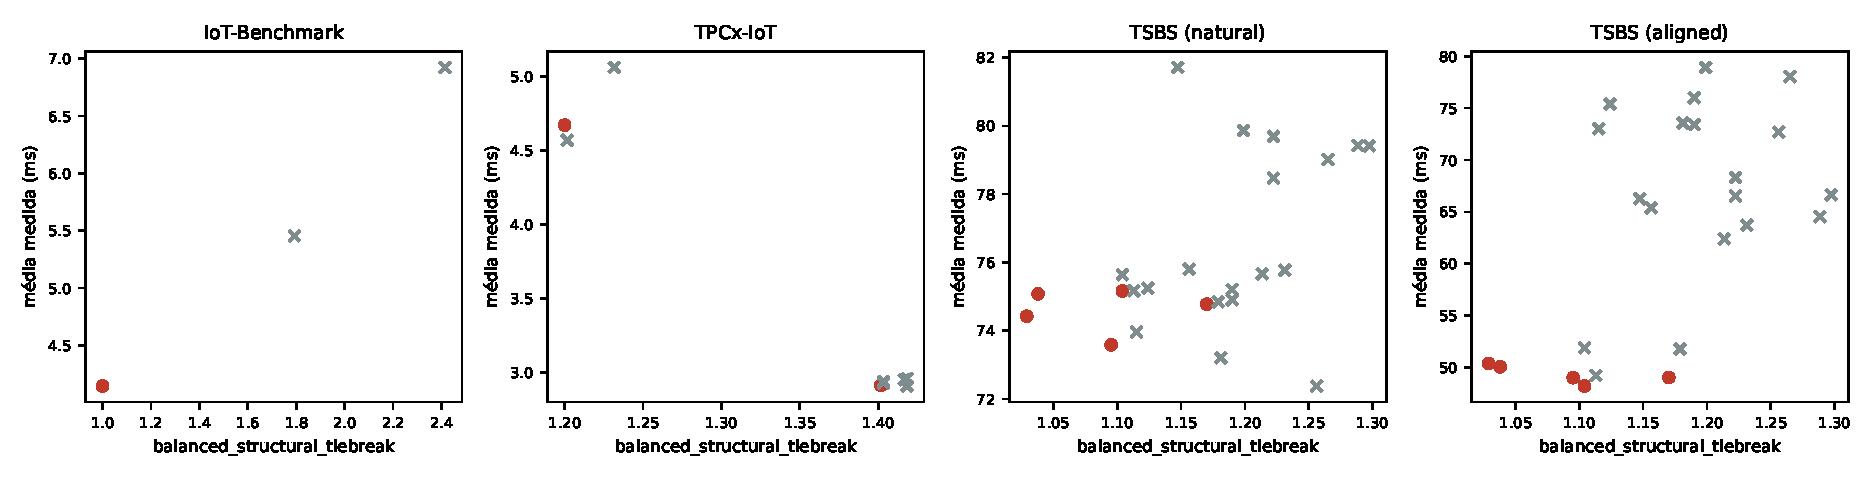
\includegraphics[width=\linewidth]{figs/tiebreak_vs_measured.pdf}
\caption{\emph{balanced\_structural\_tiebreak} contra a média medida (círculos vermelhos = HBench V3). É diagnóstico: o
desempate não pretende prever latência.}
\end{figure}
\begin{table}[H]\centering\scriptsize
\caption{RUBiS dentro do HBench V3: ordem V3 (V3H01 $\to$ V3H05) contra a medida, e o modelo NNLS da V9 aplicado depois
da campanha (\textbf{RETROSPECTIVE\_BASELINE\_ONLY}; a ordem usa os sufixos 01--05 de V3H).}
\resizebox{\linewidth}{!}{\begin{tabular}{llcrrrcrlrc}\toprule
versão & carga & melhor & empatados & piso A/A & $\tau$ V3 & Top-1 V3 & regret rank 1 & ordem NNLS & $\tau$ NNLS & Top-1 NNLS\\\midrule
\tabin{tables/rubis_within.tex}\bottomrule\end{tabular}}
\end{table}

Em resumo:
\begin{itemize}
\item O $\tau$ do desempate estrutural vai de $-0{,}34$ (TPCx) a $1{,}0$ (IoT); fica em torno de 0,35 no TSBS e em 0,8 em
três das quatro cargas do RUBiS 4.1.
\item O NNLS legado, que usa coeficientes de latência medidos, não é melhor de forma consistente: tem o mesmo $\tau$ em
três cargas e erra o Top-1 em update100x/3.11, onde o V3 acerta.
\end{itemize}
Nenhum desses números foi usado para modificar a V3.

\subsection{Ablações}
As ablações refazem a seleção sobre os vetores congelados e são avaliadas com as medições já feitas, sem nova execução
no Cassandra.

\begin{table}[H]\centering\scriptsize
\caption{Ablações: $|H|$, regret e retenção da fronteira medida. ``Sem segurança de partição'' é idêntica por
construção (os eixos de risco não entram na dominância).}
\resizebox{\linewidth}{!}{\begin{tabular}{lrrrrrrrrrrrr}\toprule
& \multicolumn{3}{c}{IoT} & \multicolumn{3}{c}{TPCx-IoT} & \multicolumn{3}{c}{TSBS natural} & \multicolumn{3}{c}{TSBS alinhada}\\
ablação & $|H|$ & regret & ret. & $|H|$ & regret & ret. & $|H|$ & regret & ret. & $|H|$ & regret & ret.\\\midrule
\tabin{tables/ablations.tex}\bottomrule\end{tabular}}
\end{table}

\begin{itemize}
\item No TPCx, o número de requisições carrega a decisão: sem ele (ou com $k=1$) sobra só TS0, com regret de 61\%.
\item No TSBS, retirar linhas, bytes ou requisições piora o regret (de 1,7\% para 2,2\%), mas aumenta a retenção.
\item $k=1$ e a escolha aleatória de $k$ são piores que a V3 nas coortes do TSBS: 2,8\% e 4,5\% com $k=1$; 3,4\% e 7,4\% na
escolha aleatória.
\item No RUBiS só o HBench foi medido, então as ablações que trocam membros não são avaliáveis.
\end{itemize}

\subsection{Reprodutibilidade entre sessões (RUBiS)}
\begin{table}[H]\centering\scriptsize
\caption{Mesmo deployment medido na sessão V2 e na sessão V3 (4.1.12).}
\begin{tabular}{lllrrr}\toprule carga & V3 & V2 & V3 (ms) & V2 (ms) & razão\\\midrule
\tabin{tables/rubis_repro.tex}\bottomrule\end{tabular}
\end{table}
As razões vão de 0,85 a 1,22. A conclusão qualitativa (H01 mais rápido que NoSE e QPG) se repete; diferenças
menores que o piso A/A não são interpretáveis entre sessões.

% =====================================================================
\section{Discussão}
\label{sec:discussao}

\paragraph{Preservação.}
O resultado central é positivo. Com a mesma semântica nos quatro benchmarks, a V3 reduziu os espaços em 67\% a 98\% e
manteve, em todos os casos, um deployment igual ao melhor medido ou empatado com ele dentro do denominador declarado:
\begin{itemize}
\item IoT: 1 de 3;
\item TPCx: 2 de 9;
\item TSBS: 5 de 24;
\item RUBiS: 5 de 256 viáveis, com preservação afirmada contra os baselines.
\end{itemize}
A V3 conseguiu isso sem fator por família e sem latência calibrada. A V2 obtinha preservação semelhante com mais
deployments (redução de 0\% a 44\% nos mesmos denominadores).

\paragraph{Ranking.}
A ordem estrutural não prediz latência, como esperado pelo desenho. Os casos de bom $\tau$ (IoT; RUBiS em leitura)
coincidem com diferenças grandes no número de requisições, e os de $\tau$ ruim (TPCx, TSBS natural) com espaços em que
muitos deployments empatam pelo ruído. Um $\tau$ ruim é um resultado, não um defeito a corrigir depois de olhar os
dados.

\paragraph{Escrita e armazenamento.}
A dominância penaliza mutações e armazenamento lógico, o que explica as escolhas mais enxutas:
\begin{itemize}
\item TPCx: TS0 em primeiro lugar;
\item TSBS: ausência das variantes com TS5sc e TS1;
\item RUBiS: H01 antes de H02.
\end{itemize}
O armazenamento medido acompanha a ordem do proxy lógico dentro de cada benchmark.

\paragraph{Onde a V3 perdeu.}
\begin{enumerate}
\item A retenção da fronteira medida de três objetivos cai no TPCx (de 83\% para 33\%), porque a V3 é mais seletiva e os
eixos estruturais não distinguem deployments que empatam na leitura.
\item A diversidade estrutural mantém variedade de projeto, não desempenho: V3H05 é lento.
\item A regra de rota lexicográfica prefere uma requisição a seis vezes mais linhas (D-V3-008). Ela não foi ajustada.
\end{enumerate}

% =====================================================================
\section{Limitações}
\label{sec:limites}
\begin{itemize}
\item O trabalho estrutural não modela cache, compactação nem custo por requisição do \emph{driver}.
\item LBP-1 não inclui \emph{overhead} de célula nem compressão.
\item As contagens de linhas do RUBiS são esperanças (aproximação de independência da síntese de rotas da V9), e não
contagens exatas por requisição como no TSBS.
\item IoT e TPCx não tiveram sessão V3 independente (reutilização por instrução do projeto, D-V3-001).
\item No RUBiS os 256 deployments viáveis não foram medidos; a preservação vale dentro do conjunto medido.
\item Os pisos A/A são altos em parte das células: 12,3\% no TSBS natural e 22--23\% no RUBiS 4.1 browsing e update100x.
\item Escala pequena, nó único e RF~1.
\item Desvio declarado do TSBS (2 + 12 rodadas).
\item Outros contêineres Cassandra permaneceram ativos no servidor, isolados por cpuset e pela guarda de isolamento.
\end{itemize}

% =====================================================================
\section{Reprodução}
\begin{verbatim}
./run_v3_unified.sh --audit         # git, docker, digest do protocolo
./run_v3_unified.sh --prebenchmark  # Stage 7/8 V3 + docs/V3_PREBENCHMARK_COMPARISON.md
./run_v3_unified.sh --test          # 15 testes obrigatórios (41 casos)
./run_v3_unified.sh --freeze        # SHA-256 + PREREGISTRATION_V3.json
./run_v3_unified.sh --benchmark     # reuso IoT/TPCx; TSBS e RUBiS desacoplados
./run_v3_unified.sh --analyze       # métricas, ablações, NNLS retrospectivo
versao_ajustada/.venv/bin/python artigo_overleaf_v3/build_tables.py
\end{verbatim}
{\sloppy Artefatos: \texttt{outputs\_v3/<benchmark>/} \texttt{\{prebenchmark, benchmark, analysis\}}. Decisões: \texttt{docs/V3\_DECISION\_LOG.md}
(D-V3-001 a D-V3-015, todas anteriores à medição). Os \emph{traces} brutos do RUBiS (2,2~GB) estão fora do git, com
SHA-256 registrado em \texttt{outputs\_v3/rubis/benchmark/run1/RAW\_SHA256.json}.\par}

\end{document}
